\chapter{Implementación} \label{ch:results}

\indent Este capítulo tiene como objetivo mostrar y reflejar el trabajo hecho. El preprocesamiento y el
procesamiento se ha explicado en capítulos anteriores. Aquí se mencionarán los elementos necesarios para la ejecutar
la clasificación, como por ejemplo el \textit{framing}. Se describirá la arquitectura de la red \gls{lstm}
utilizada, junto a la descripción de sus capas intermedias y los hiperparámetros seleccionados. \bigskip

\subsection*{Diagrama de flujo del sistema} \label{subsec:flow-diagram}

\indent Antes de abordar cada uno de los distintos pasos, se ilustra una diagrama de flujo de todo el sistema.
Empezando desde el filtrado lineal para eliminar ruido que corrompa la señal, pasando por la extra cción de marcas y
la extracción de atributos para dar finalmente con la clasificación de los estados de la señal (diagrama que
contempla tanto la etapa de entrenamiento como la de evaluación).


\begin{figure}[H]
  \centering
  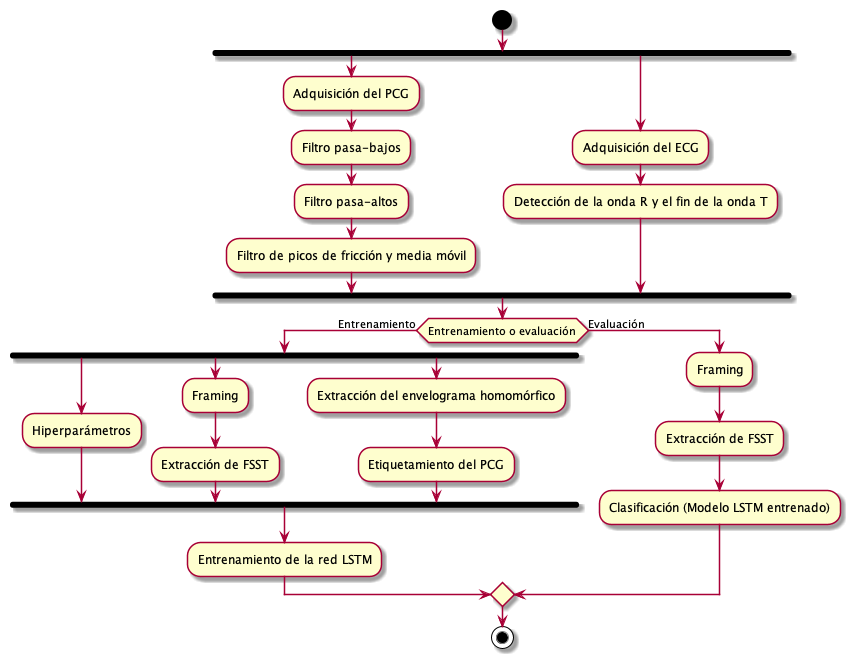
\includegraphics[scale=0.7]{sections/chapter-07/images/flow-diagram.png}
  \caption[Diagrama de flujo del sistema]{Diagrama de flujo del sistema.}
  \label{fig:flow-diagram}
\end{figure}

\newpage

\section{Encuadrado} \label{sec:framing}

\indent El proceso de dividir una señal de una dada longitud $L$ en señales de igual longitud se denomina encuadrado
(\textit{framing}). Ésto es necesario debido a que las señales de fonocardiograma poseen longitudes diferentes. La
base de datos, ya se ha mencionado, tienen adquisiciones de distintas duraciones, y la arquitectura propuesta más
adelante, necesita como entrada $M$ señales con una longitud $N$ fija. \\
\indent El encuadrado es posible realizarlo con una ventana cuadrada, o cualquier otro tipo de ventana. La elección
de la ventana esta dada por el problema a resolver. En este caso, se utilizó una ventana cuadrada. \bigskip

\indent Dada una señal $\mathbf{x} \in \mathbb{R}^T$, se desea obtener una cantidad $Q$ de señales. Este valor está
dada por la ecuación \ref{eq:q}

\begin{align}
  \label{eq:q}
  Q := \left[\frac{T-1-N}{\tau}\right]
\end{align}

\indent La notación $[...]$ implicá el entero más cercano. El deslizamiento de la ventana está dado por $\tau$,
dependiendo de $N$ y de $\tau$, se define si existe solapamiento u \textit{overlapping}.

\begin{align}
  O =
  \begin{cases}
    1, \; 0 \leq \tau \leq N \\
    0, \; \tau \geq N
  \end{cases}
\end{align}

\indent De esta manera, queda definido el vector, $\bm{\Tilde{x}}_k \in \mathbb{R}^{N}$ según la siguiente ecuación.

\begin{align}
  \bm{\Tilde{x}}_k = \left[\begin{array}{cccc}
    \bm{x}_{\tau \cdot k} &
    \bm{x}_{\tau \cdot k+1} &
    \dots & \bm{x}_{\tau \cdot k + N - 1}
  \end{array}\right]^\top
\end{align}

\begin{align}
  \bm{X}_j = \left[\begin{array}{cccc}
    \bm{\Tilde{x}}_1 &
    \bm{\Tilde{x}}_2 &
    \dots &
    \bm{\Tilde{x}}_Q
  \end{array}\right]^\top
\end{align}

\indent Donde $k = 1,2,...,Q$. Por último, una vez obtenidos los $Q$ cuadros para una señal $j$, donde $j = 1,2,...,
D$ y $D$ la cantidad total de señales, se itera sobre todo el set de datos y se genera la matriz $\bm{H} \in
\mathbb{R}^{M \times N}$.

\begin{align}
  \bm{H} = \left[\begin{array}{cccc}
    \bm{X}_1 &
    \bm{X}_2 &
    \dots &
    \bm{X}_D
  \end{array}\right]^\top
\end{align}

\indent Es importante tener en cuenta que en los casos que $\frac{T-1-N}{\tau}$ no sea entero, quedarán muestras
(generalmente del final) sin incluir en los datos, las cuales serán descartadas.

\section{Extracción de atributos}

\indent Una vez hecho el acondicionamiento de la señal (filtrado, normalización en términos de energía) y los
cuadros listos, se procede a extraer los features necesarios a introducir al clasificador. Los features extraídos
son obtenidos por medio de la \gls{fsst}, el clasificador es una red diseñada con celdas \gls{lstm}. \bigskip

\indent Para la extracción de features en tiempo-frecuencia se utilizó la \gls{fsst}. Esta se aplica sobre
segmentos de señal extraídos del proceso de encuadrado. \\
\indent En esta ocasión, no se utiliza solapamiento de cuadros (\textit{frames}), con lo cual cada segmento de señal
posee información única a excepción de una muestra. Previamente, se eligen las señales mayores o iguales a una
longitud $N$, cuyo valor va a ser el largo de cada segmento. \\
\indent A cada segmento se le aplica la transformada con una ventana definida. La ventana elegida es la ventana de
Kaiser con una longitud $L = 128$ y un $\beta = 0.5$. Esta ventana fue seleccionada dado a que su objetivo es
maximizar la relación de energía entre lóbulo principal y sus lóbulos secundarios, reduciendo los efectos del ruido
en esas bandas de frecuencia y mejorando la calidad de la transformada.

\begin{figure}[H]
  \centering
  \begin{subfigure}{\textwidth}
    \centering
    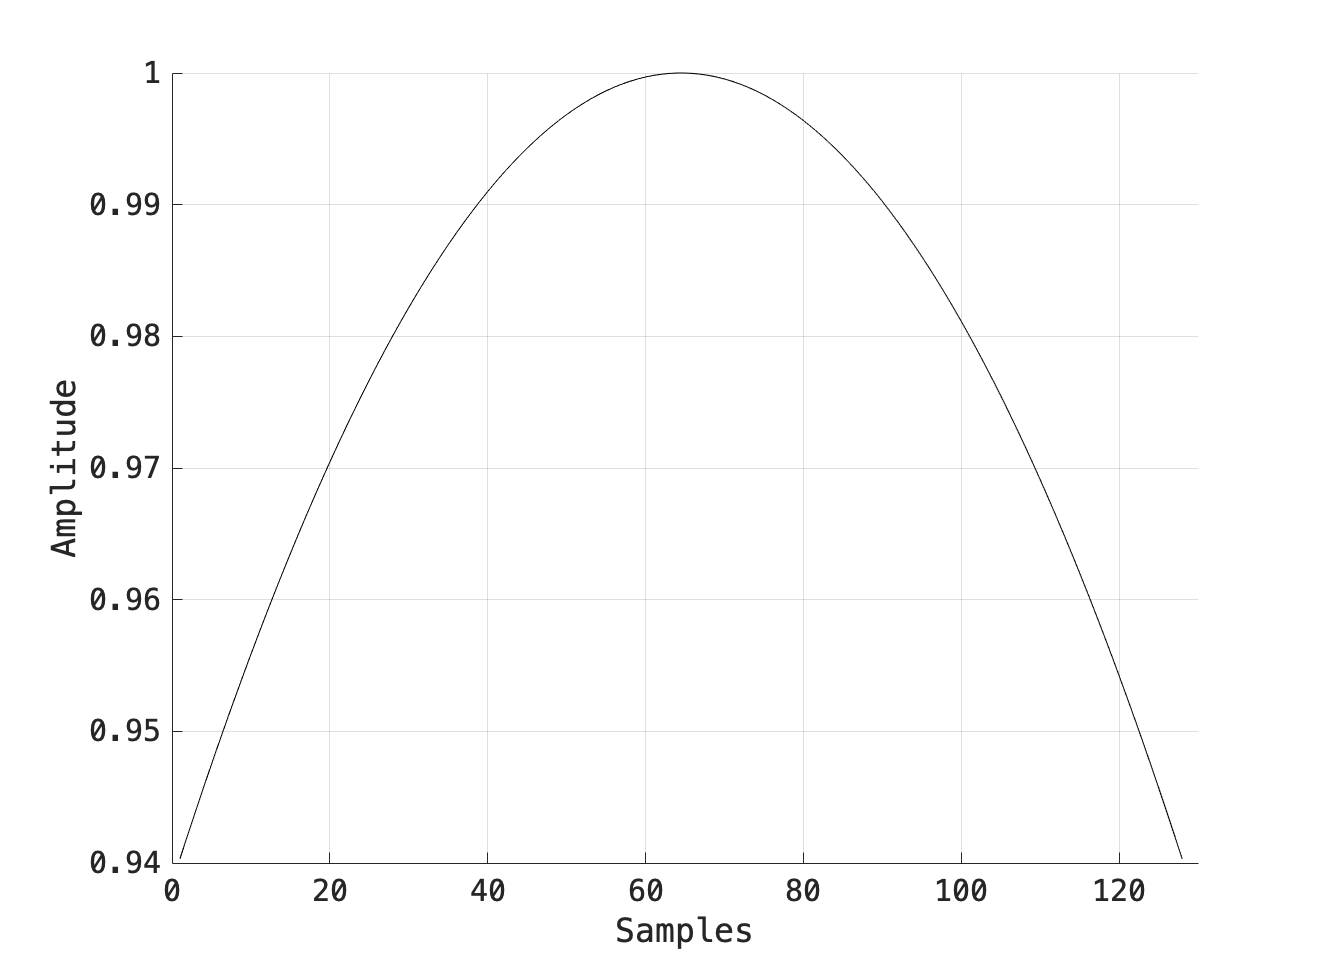
\includegraphics[scale=0.23]{sections/chapter-07/images/kaiser-window.png}
    \caption[Ventana de Kaiser]{Ventana de Kaiser. La ventana diseñada con un largo $L = 128$ y un $\beta = 0.5$.}
  \end{subfigure} \\
  \begin{subfigure}{\textwidth}
    \centering
    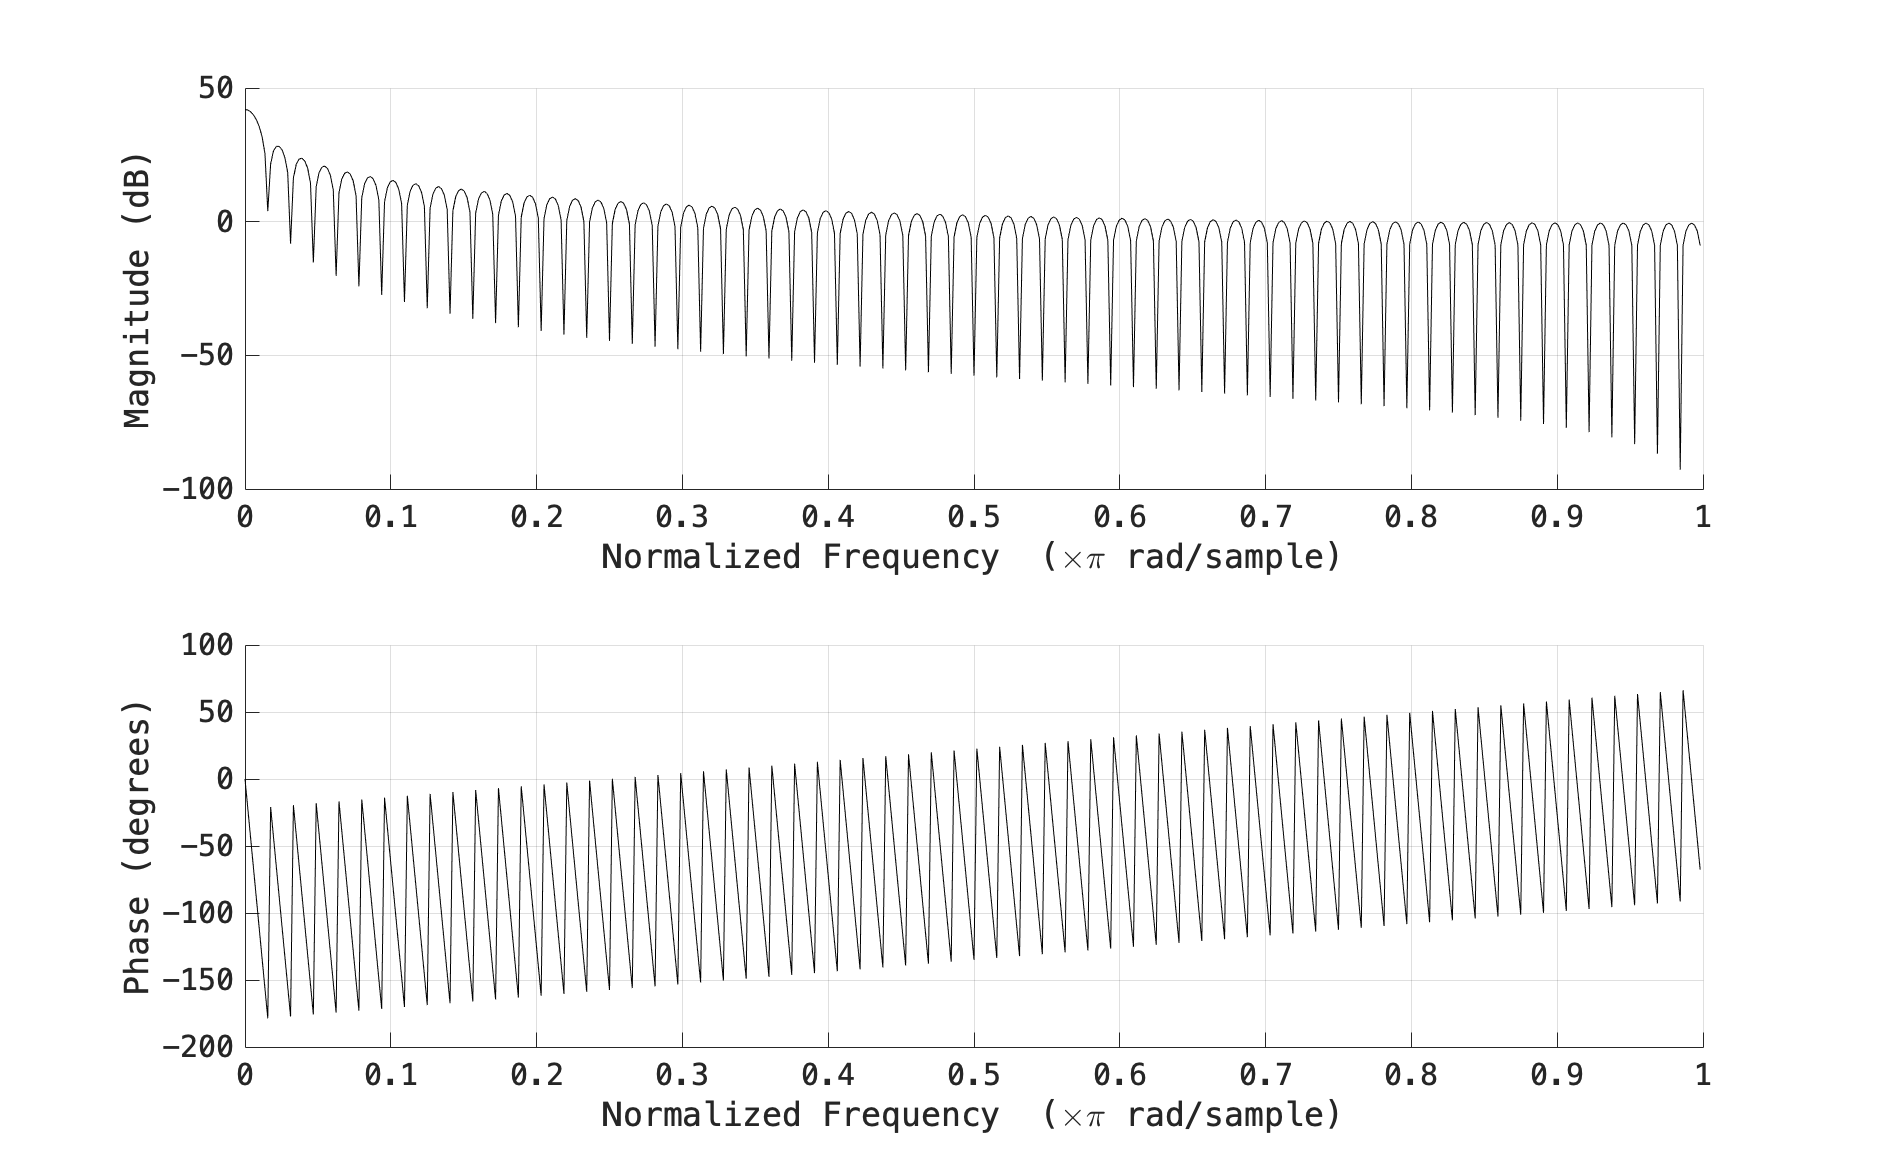
\includegraphics[scale=0.21]{sections/chapter-07/images/kaiser-window-freqz.png}
    \caption[Respuesta en frecuencia de la ventana de Kaiser]{Respuesta en frecuencia de la ventana de Kaiser. La
    respuesta se encuentra en decibeles y se ilustra tanto la magnitud como la fase.}
  \end{subfigure}
  \label{fig:kaiser-window-plot}
\end{figure}

\indent El parámetro $\beta$ se calcula en base a la ecuación \ref{eq:kaiser-beta}.

\begin{align} \label{eq:kaiser-beta}
  \beta = \begin{cases}
    0.1102(\alpha-8.7), \; \alpha > 50 \\
    0.5842(\alpha-21)^{0.4}+0.7886(\alpha-21), \; 50 \geq \alpha \geq 21, \\
    0, \; \alpha \geq < 21
  \end{cases}
\end{align}

Y la banda de transición, según el largo de la ventana, se calcula despejando $\Delta\omega$ de la ecuación
\ref{eq:kaiser-transition-band}.

\begin{align} \label{eq:kaiser-transition-band}
  L = \frac{\alpha-8}{2.285\Delta\omega} + 1
\end{align}

\indent En la Figura \ref{fig:pcg-fsst} se ilustra la transformada extraída de una señal de fonocardiograma. Se
visualiza claramente el contenido frecuencia en los distintos sonidos del fonocardiograma y la periodicidad de los
mismos. Por otro lado, se muestra que por debajo de frecuencias de los 20 Hz y por encima de los 200 Hz no hay
contenido espectral relevante en cuanto a energía. La mayor cantidad de contenido frecuencia se encuentra entre
dicho rango. Por ende, se extraen los features entre 20-200 Hz como entrada al clasificador.

\begin{figure}[H]
  \centering
  \begin{subfigure}{\textwidth}
    \centering
    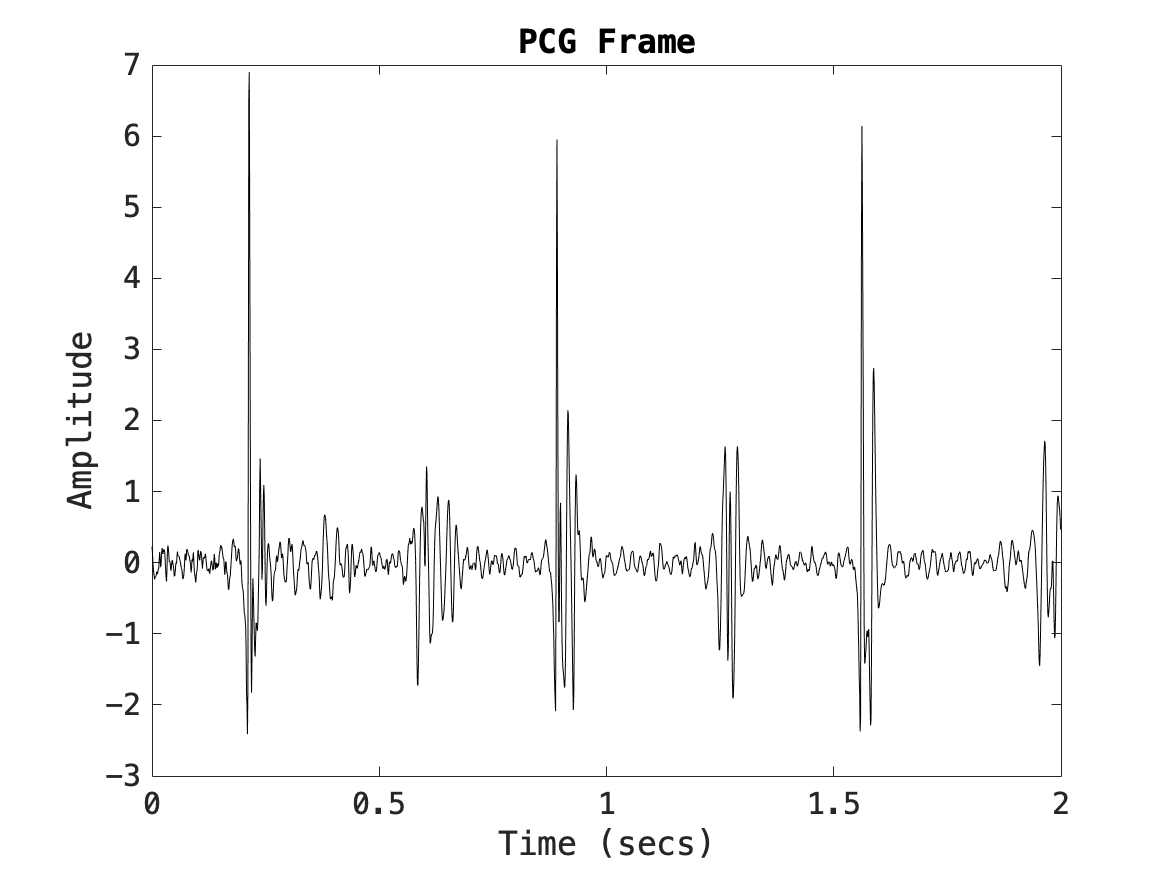
\includegraphics[scale=0.27]{sections/chapter-07/images/pcg-frame.png}
    \caption[Segmento de una señal de fonocardiograma]{Segmento de una señal de fonocardiograma.}
    \label{fig:pcg-frame}
  \end{subfigure} \\
  \begin{subfigure}{\textwidth}
    \centering
    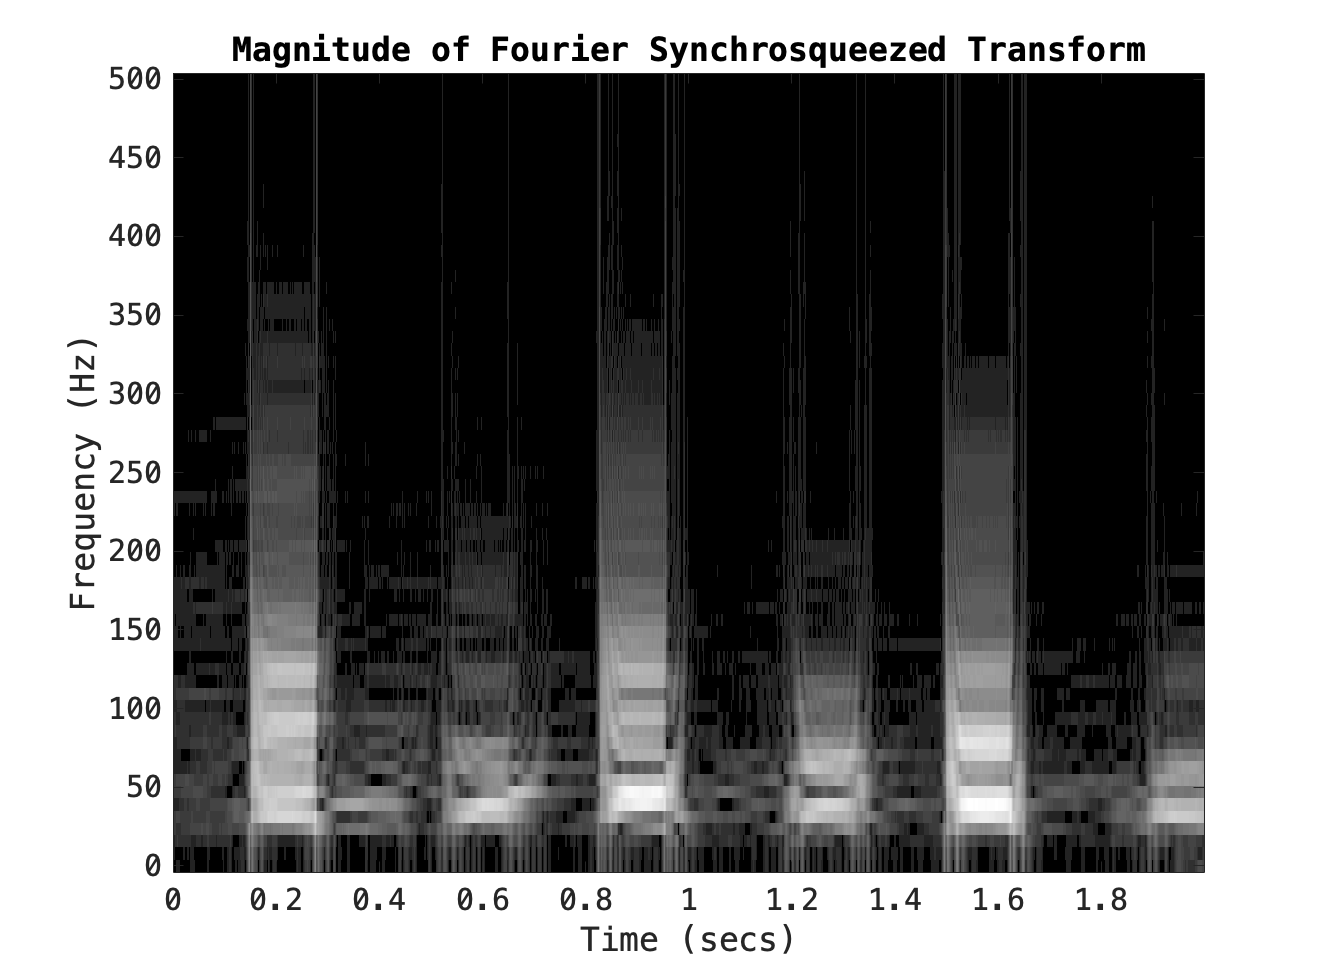
\includegraphics[scale=0.25]{sections/chapter-07/images/fsst-plot.png}
    \caption[Magnitud de la \gls{fsst} aplicada a un segmento de señal de fonocardiograma]{Magnitud de la
    \gls{fsst} aplicada a un segmento de señal de fonocardiograma.}
    \label{fig:fsst-diagram}
  \end{subfigure}
  \caption[Ejemplo de la transformada \gls{fsst} a un segmento de señal de \gls{pcg}]{Ejemplo de la
  transformada \gls{fsst} a un segmento de señal de \gls{pcg}.}
  \label{fig:pcg-fsst}
\end{figure}

\indent Se ve claramente como la mayor energía frecuencial corresponde a los instantes donde se producen los sonidos
fundamentales. También, en este ejemplo, hay energía proveniente de otras fuentes de ruido, entre los instantes 1-1
.2 segundos.

\subsection{Modelo} \label{subsec:model}

\indent El clasificador es una red neuronal \gls{lstm} como se ha mencionado anteriormente. Los parámetros a
estimar del modelo pertenecen a la capa \gls{lstm}. Por otro lado, es predefinir los hiperparámetros de la red
neuronal. Además de la capa recurrente, a una red neuronal la componen otras capas intermedias y una capa de entrada
y salida.

\subsubsection{Arquitectura}

\indent La arquitectura de la red neuronal consiste en de 5 capas. Una de entrada, una recurrente, una
\textit{fully-connected} con otra de softmax y una de salida. La arquitectura se ilustra en la Figura
\ref{fig:nn-architecture}.

\begin{figure}[H]
  \centering
  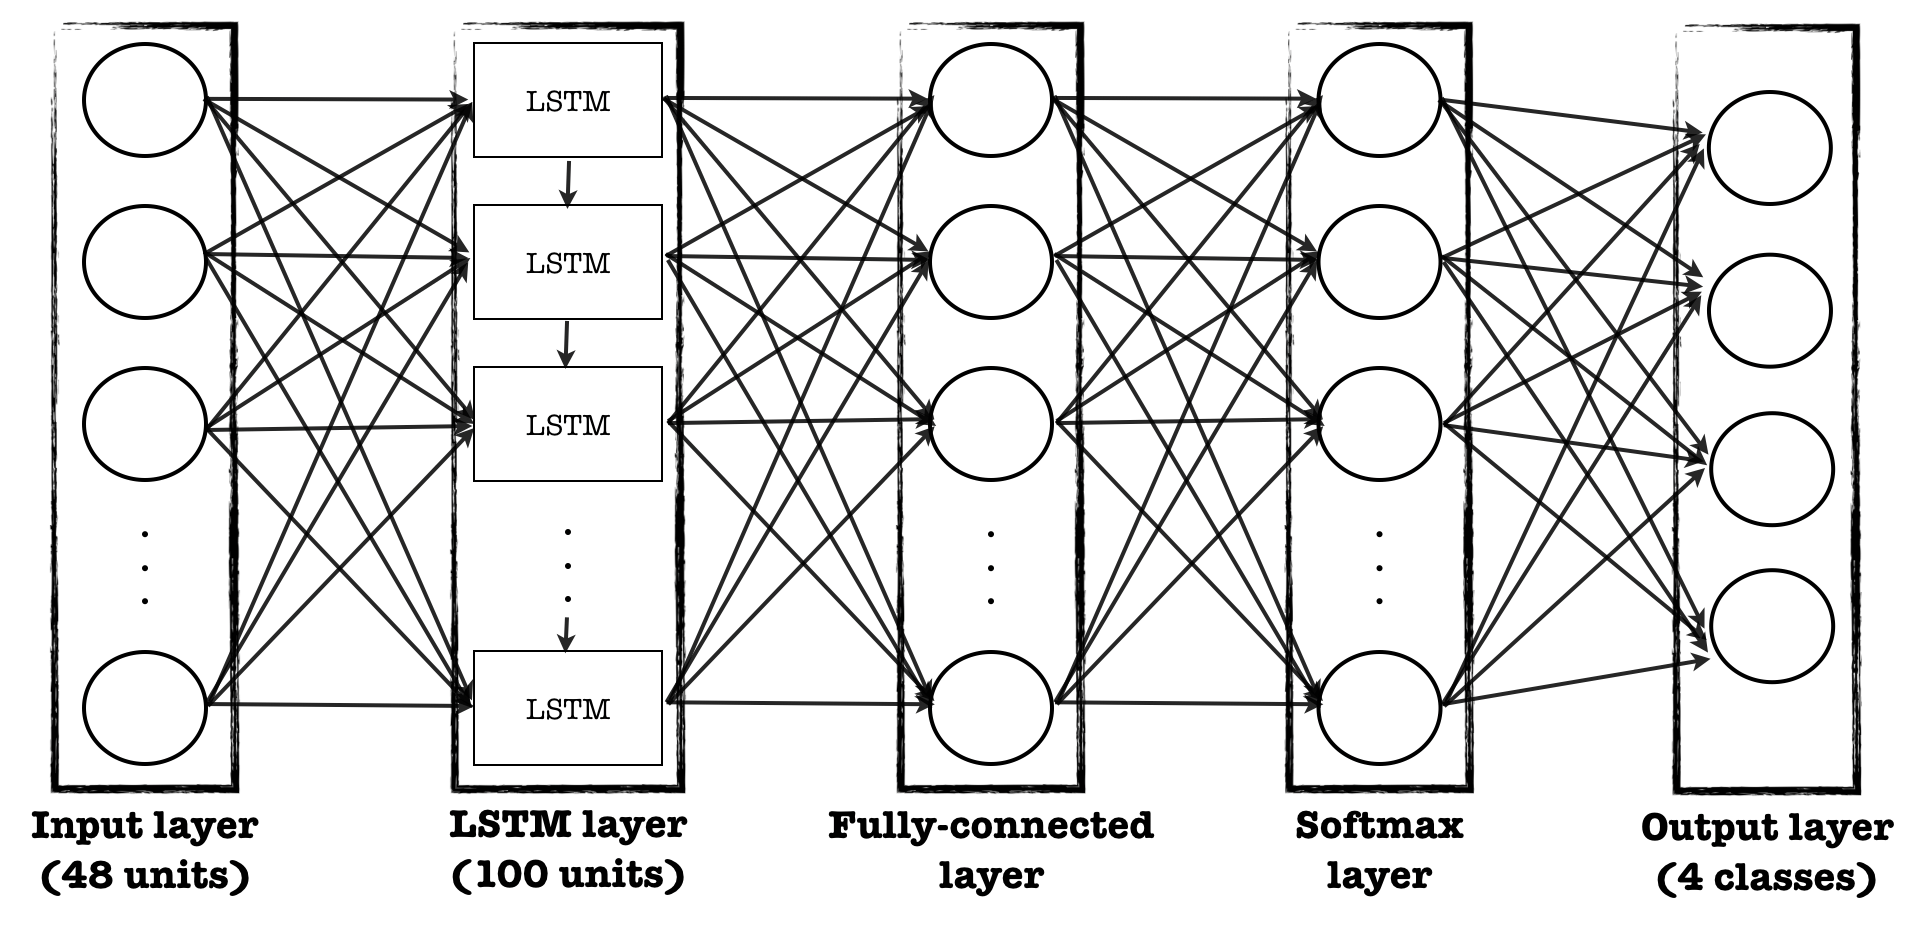
\includegraphics[scale=0.35]{sections/chapter-07/images/lstm-architecture.png}
  \caption[Arquitectura de la red neuronal]{Arquitectura de la red neuronal.}
  \label{fig:nn-architecture}
\end{figure}

\subsubsection{Hiperparámetros}

\indent Ya se ha visto que es necesario establecer hiperparámetros de la red. Para el entrenamiento se utiliza el
algortimo publicado en 2014 en la \gls{iclr} 2015, denominado \textit{Adam} \cite{pp:adam}. El algoritmo
introduce ciertos hiperparámetros además de los convencionales que es necesario definir a priori. \\*
\indent Los hiperparámetros utilizados en la implementación se listan a continuación \footnote{Los nombres de los
hiperparámetros se encuentran en inglés, dado a que no hay literatura en español y muchos de ellos no tienen
traducción}.

\begin{itemize}
  \item \texttt{MaxEpochs: 10}
  \item \texttt{MiniBatchSize: 50}
  \item \texttt{InitialLearngRate: 0.01}
  \item \texttt{LearnRateDropPeriod: 3}
  \item \texttt{LearnRateDropFactor: 0.1}
  \item \texttt{L2Regularization: 1e-04}
  \item \texttt{GradientDecayFactor: 0.9}
  \item \texttt{SquaredGradientDecayFactor: 0.99}
  \item \texttt{Epsilon: 1e-08}
  \item \texttt{GradientThreshold: 1}
\end{itemize}

\indent Generalmente, lo normal es elegir la cantidad de \textit{epochs} alrededor de 10. En disintas aplicaciones
se han utilizado un número entre $15-30$. Esto hace que el tiempo de entrenamiento sea aún mayor. Recordar que por
cada una de ellas todo el set de datos ha pasado por la red. Por temas de cómputo y tiempos, se decidió fijar la
cantidad de \textit{epochs} en el valor estándar. Por otro lado, bastante ligado a la cantidad de \textit{epochs} y
el tamaño del lote se definió por motivos computacionales, tiempo y desempeño de la red por medio de distintas
iteraciones. \\
\indent Otros parámetros de interés, son \textit{InitialLearnRate}, \textit{LearnRateDropPeriod} y
\textit{LearnRateDropFactor}. Éstos son necesarios dado a que el \textit{LearnRate} se modifica a lo largo de las
iteraciones, y con estos parámetros se define cada cuánto y por cuánto se reduce el mismo. En esta implementación se
definió que cada 3 \textit{epochs} se reduce un 1\%. \\
\indent Lo que se conoce como \textit{Regularization} intenta resolver el problema de generalización o
sobreentrenamiento en lo que respecta a los pesos de la red. También se lo denomina, en inglés, \textit{weight
decay}. Estos pesos se encuentran asociados a la función de costo y \textit{L2Regularization} se encuentra
representado como un factor. En esta implementación toma el valor de 1e-04. La función de costo, $E_R(\theta)$, con
el factor de regularización tiene la forma de la ecuación \ref{eq:l2-regularization}.

\begin{align} \label{eq:l2-regularization}
E_R(\theta) = E(\theta) + \lambda \Omega(w)
\end{align}

Donde,

\begin{align}
  \Omega(w) = \frac{1}{2} w^\top w
\end{align}

\indent $\Omega(w)$ es la función de regularización y $w$ son los pesos, la cual se encuentra multiplicada por el
factor $\lambda$ correspondiente a \textit{L2Regularization}. \bigskip

\indent Luego, los factores inherentes al algoritmo Adam, son \textit{GradientDecayFactor} y
\textit{SquaredGradientDecayFactor}. Normalmente en la mayoría de los casos toman el valor de $0.9$ y $0.99$
respectivamente. \\
\indent Adam utiliza medias móviles para actualizar los parámetros de la red. Estas medias se utilizan para el
gradiente y el gradiente al cuadrado, según las ecuaciones \ref{eq:gradient}, \ref{eq:squared-gradient}.

\begin{align} \label{eq:gradient}
  m_l = \beta_1 m_{l-1} + (1-\beta_1) \nabla E(\theta_l)
\end{align}

\begin{align} \label{eq:squared-gradient}
  v_l = \beta_2 v_{l-1} + (1-\beta_2) [\nabla E(\theta_l)]^2
\end{align}

Donde, $\beta_1$ y $\beta_2$ son los hiperparámetros \textit{GradientDecayFactor} y \textit{SquaredGradientDecayFactor}.

\begin{align} \label{eq:adam-update}
  \theta_{l+1} = \theta_l + \frac{\alpha m_l}{\sqrt{v_l}+\epsilon}
\end{align}

\indent La ecuación \ref{eq:adam-update} define cómo se actualizan los parámetros de la red con las medias móviles.
Por otro lado, si los gradientes durante varias iteraciones son similares, el uso de las medias móviles de los
gradientes permiten a la actualización de los parámetros tomar momento hacia una dirección. Existe la posibilidad de
que los gradientes sólo contengan ruido con lo cual, las medias móviles de los gradientes serán pequeñas y así
también actualización. Para ellos se elige un valor $\epsilon$ tal que la actualización esa no diverja, ya que
$\sqrt{v_l}$ puede ser muy pequeño. En muchas ocasiones se utiliza $\epsilon = 0.01$ pero en aplicaciones un valor
cercano a 1 funciona mejor. Queda definir el parámetro $\alpha$ como el \textit{LearnRate} mencionado. Es posible
que este parámetro tome diferentes valores para distintas capas intermedias y depende del algoritmo en cuestión. Es
por eso que no se puede definir un valor estándar de este hiperparámetro. \bigskip

\indent Por último, queda definir el hiperparámetro \textit{GradientThreshold}. Este umbral intenta acortar el
gradiente si los valores lo exceden. El método se basa en utilizar la norma L2 tal que si la norma del gradiente
excede el umbral, se escala el gradiente tal que su norma lo igual. En este caso el umbral toma el valor de 1.

\subsection{K-Folds} \label{subsec:k-folds}

\indent Recoradar que la técnica utilizada para resolver el problema de generalidad en el momento del entrenamiento
es la ya mencionada en el Capítulo \ref{ch:deep-learning}, validación cruzada (particularmente
\textit{10-Folds}). Para separar los fonocardiogramas en distintos grupos, se define el siguiente algoritmo. \bigskip

\indent Sea la señal de fonocardiograma $\mathbf{s}_i \in \mathbb{R}^N$, sus etiquetas (previamente calculadas)
$\mathbf{l}_i \in \mathbb{R}^N$ y la cantidad de \textit{folds} $K$. La cantidad de fonocardiogramas está dada por
el valor $L$, por lo tanto $i = 0,1,2,\dots,L-1$. \bigskip

\indent De esta manera se define $M$ como la cantidad de \gls{pcg} por \textit{fold}.

\begin{align}
  M = \left\lfloor \frac{L}{K} \right\rfloor
\end{align}

\indent Por lo tanto la ecuación \ref{eq:fold-selection} define cómo asignar cada \gls{pcg} a un \textit{fold}.

\begin{align} \label{eq:fold-selection}
 F_{n,j} = i, \quad (n \cdot M) < i < (n+1) \cdot (M-1)
\end{align}

\indent Con $i=0,1,2,\dots,M-1$ y $n = 0,1,2,\dots,K-1$. De esta manera se define la matriz $\bm{F} \in
\mathbb{R}^{K \times M}$, que contiene los indices correspondientes a cada \textit{fold}.

\begin{align}
  \bm{F} = \left[\begin{array}{ccccc}
    F_{0,0} & F_{0,1} & \dots & F_{0,M} \\
    F_{1,0} & F_{1,1} & \dots & F_{1,M} \\
    \vdots  & \vdots  & \ddots & \vdots \\
    F_{K,0} & F_{K,1} & \dots & F_{K,M}
  \end{array}\right]
\end{align}

\indent Si $\frac{L}{K}$ no fuese un número entero, significaría que no todos los \textit{folds} contendrán la misma
cantidad. La cantidad de señales huérfanas se calcula en la ecuación \ref{eq:pcg-lefts}.

\begin{align} \label{eq:pcg-lefts}
  L_{s} = \mathrm{mod}(L,K)
\end{align}

\indent En este momento es cuando se decide eliminar esas señales, agregar más para que la matriz $\mathbf{F}$ sea
consistente o se agregan de manera aleatoria a cualquier \textit{fold}.

Para definir los distintos grupos, los cuales serán $K$, cada grupo contenerá $K-1$ folds de entrenamiento y 1
\textit{fold} de evaluación. \\
\indent Se definen la matriz de entrenamiento, $\bm{T}_p \in \mathbb{R}^{K-1 \times M}$ y la matriz de evaluación
$\mathbf{E}_p \in \mathbb{R}^M$. Ambos asociados a un grupo $P \in \{0,1,2,\dots,K-1\}$

\begin{align}
  \mathrm{fil}_i(\bm{T}_p) = \mathrm{fil_j(\bm{F})}, \quad j \in \{0,1,2,\dots,K-1\}-\{p\}
\end{align}

\begin{align}
  \bm{E}_{p} = \mathrm{fil_p}(\bm{F})
\end{align}

\indent De esta manera, quedan definidos los grupos para realizar los K entrenamientos y ponderar métricas de
performance.

\section{Clasificación}

\indent La clasificación se realiza a partir de las probabilidades de la matriz $\bm{B} \in \mathbb{R}^{n \times 4}$.
Esta matriz es la que la capa de salida genera. En ella la se encuentra la probabilidad de que cada muestra de la
señal pertenezca a alguna clase. La forma de elegir la clase se muestra en la ecuación \ref{eq:class-definition}.
Esto es lo que generalmente la mayoría de las redes neuronales a su salida realizan como forma de clasificación, es
el caso de la segmentación mediante la una adaptación de la red neuronal \textit{U-Net} de Renna \textit{et al.}
\cite{pp:renna2018}.

\begin{align} \label{eq:class-definition}
C_i = \arg \underset{j}{\mathrm{max}} \; B_{i,j}
\end{align}


\indent Es necesario mencionar que en el entrenamiento de la red neuronal no se ha impuesto ninguna restricción de
transición de estados, a diferencia de lo que realmente sucede en el fonocardiograma. De esta manera, existen en la
predicción y por ende en la clasificación transiciones espurias que no corresponden. En la Figura
\ref{fig:spurious-transitions} se ilustra este fenómeno.

\begin{figure}[H]
  \centering
  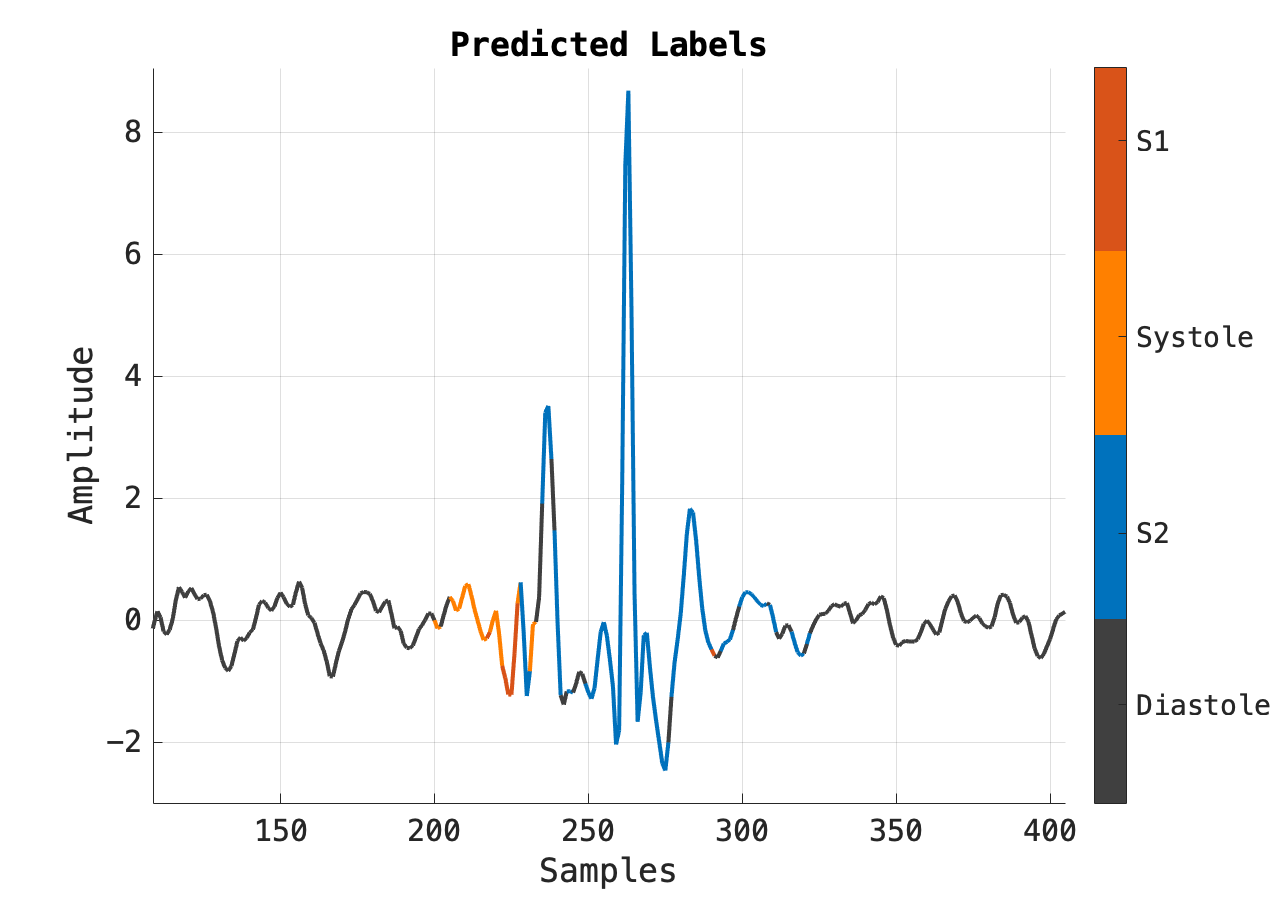
\includegraphics[scale=0.3]{sections/chapter-07/images/predicted-labels.png}
  \caption[Etiquetas predecidas por la red]{Etiquetas predecidas por la red.}
  \label{fig:spurious-transitions}
\end{figure}

\indent Para corregir la transición de estado espúrios los posteriores capítulos se propondrán algunas técnicas.
Esto ayudará a la efectividad de la detección y para mantener la consistencia de los estados. Este ruido no es
deseado en algoritmos que utilicen las transiciones del fonocardiograma.
